Relative weights of a 2-site system:
\begin{align*}
	\left\langle W\right| E E \left| V\right\rangle&=\frac{1}{\alpha^2}\left\langle W|V\right\rangle & \left\langle W\right| ED\left|V\right\rangle&=\frac{1}{\alpha\beta}\left\langle W|V\right\rangle\\
	\left\langle W\right| DE\left|V\right\rangle &=\left\langle W\right| D+E\left|V\right\rangle = \left(\frac{1}{\alpha}+\frac{1}{\beta}\right)\left\langle W | V\right\rangle & \left\langle W \right| DD \left| V\right\rangle &= \frac{1}{\beta^2}\left\langle W| V\right\rangle
\end{align*}
We already expressed the current of a $N$-site system by 
\begin{equation*}
	J_N=\frac{Z_{N-1}}{Z_N}=\frac{\left\langle W | C^{N-1}|V\right\rangle}{\left\langle W | C^N | V \right\rangle}
\end{equation*}
It is therefore the most importent task to compute an exact expression for $C^N$, i.e. to express the sum in "{}normal order"{}. The derivation of the exact result is difficult and won't be given here. Instead we will simply quote the result:
\begin{align*}
	(D+E)^N&=\sum\limits_{p=1}^N p\frac{(2N-1-p)!}{N!(N-p)!}\sum\limits_{q=0}^pE^qD^{p-q}\\
	\leadsto \frac{\left\langle W|C^N|V\right\rangle}{\left\langle W|V\right\rangle}&=\sum\limits_{p=0}^Np\frac{(2N-p-1)!}{N!(N-p)!}\frac{\beta^{-p-1}-\alpha^{-p-1}}{\beta^{-1}-\alpha^{-1}}
\end{align*}
For infinite systems ($N\to\infty$), we get:
\begin{equation*}
	J=\begin{cases} \frac{1}{4} & \alpha\geq\frac{1}{2};\ \beta\geq\frac{1}{2} \quad \text{maximum current phase} \\ \alpha(1-\alpha) & \alpha < \frac{1}{2};\ \alpha < \beta \quad \text{low density phase} \\ \beta(1-\beta) & \beta<\frac{1}{2};\ \beta<\alpha \quad \text{high density phase} \end{cases}
\end{equation*}
\textbf{\underline{\smash{phase diagram}}}:
\begin{figure}[H]
	\centering
	\begin{tikzpicture}[>=stealth,scale=1.5]
		\draw[->] (-0.5,0)--++(2.5,0)++(0,-0.1)node[below]{$\frac{1}{2}$}--++(0,0.2)++(0,-0.1)--++(4,0)node[below right]{$\frac{\alpha}{p}$};
		\draw[->] (0,-0.5)--++(0,2.5)++(-0.1,0)node[left]{$\frac{1}{2}$}--++(0.2,0)++(-0.1,0)--++(0,2)node[above left]{$\frac{\beta}{p}$};
		\draw (0,0)--++(2,2)node[midway,below right]{$\alpha=\beta$}--++(4,0)++(-4,0)--++(0,2);
		\draw[densely dashed] (0,4)--++(2,-2)--++(-2,0)node[midway,above]{LD}++(2,0)--++(0,-2)++(0,2)--++(2,-2)node[midway,name=arrowpoint]{};
		\draw[<-] (arrowpoint) .. controls +(0.25,-0.2) and +(-0.25,0) .. ++(1,0)node[right,name=agb]{$\alpha+\beta=p$};
		\node[above right] at (arrowpoint) {HD};
		\node[name=mc] at (3,3){MC};
		\begin{scope}[xshift=-1cm,yshift=-2cm]
			\draw[->] (0,0)--(2,0)node[below right]{$x$};
			\draw[->] (0,0)--(0,1)node[above left]{$\rho(x)$};
			\draw (0,0.3)node[left]{$\alpha$} .. controls +(1.5,0.1) and +(-0.05,-0.5) .. (1.5,1)(1.5,-0.1)node[below]{$L$}--++(0,0.2);
		\end{scope}
		\draw[->] (0,-1) .. controls +(0.25,0.5) and +(0,-1) .. (0.5,1);
		\begin{scope}[xshift=2cm,yshift=-2cm]
			\draw[->] (0,0)--(2,0)node[below right]{$x$};
			\draw[->] (0,0)--(0,1)node[above left]{$\rho(x)$};
			\draw (0,0.3)node[left]{$\beta$} .. controls +(0.1,0.7) .. (2,1);
		\end{scope}
		\draw[->] (3,-0.8) .. controls +(0,0.5) and +(1,0) .. (1.5,0.5);
		\begin{scope}[xshift=4cm,yshift=3cm]
			\draw[->] (0,0)--(2,0)node[below right]{$x$};
			\draw[->] (0,0)--(0,1)node[above left]{$\rho(x)$};
			\draw[densely dashed] (0,0.5)node[left]{$\frac{1}{2}$}--++(2,0);
			\draw (0,1) .. controls +(0.1,-0.8) and +(-0.2,0.7) .. (1.4,0.1);
			\draw (1.5,-0.1)node[below]{$L$}--++(0,0.2);
		\end{scope}
		\draw[->,shorten <= 3pt,shorten >= 3pt] (4,3)--(mc);
	\end{tikzpicture} \end{figure} \noindent\textbf{\underline{\smash{The domainwall picture of the ASEP}}}\vspace{3mm}\\
The domain-wall theory describes phenomenologically the competition between two domains composed by the two reservoirs. For $\alpha<\frac{1}{2};\beta<\frac{1}{2}$ two domains coexist. The density in the left reservoir is given by $\alpha$, the flow by $\alpha(1-\alpha)$.\\
Analogously, we have a density $(1-\beta)$ and a flow $\beta(1-\beta)$ for the right domain. The two domains are separated by a shock:
\begin{figure}[H]
	\centering
	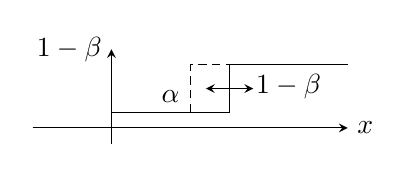
\begin{tikzpicture}[>=stealth]
		\draw[->] (0,-0.2)--(0,1)node[left]{$1-\beta$};
		\draw[->] (-1,0)--(3,0)node[right]{$x$};
		\draw (0,0.2)--(1.5,0.2)node[midway,above]{$\alpha$}--++(0,0.6)--++(1.5,0)node[midway,below]{$1-\beta$};
		\draw[<->] (1.2,0.5)--(1.8,0.5);
		\draw[densely dashed] (1,0.2)--++(0,0.6)--(1.5,0.8);
	\end{tikzpicture}
\end{figure}
\noindent The domain wall is displaced to the left by the particle from left reservoir. The displacement is given by:
\begin{equation*}
	\Delta m=J_\alpha \Delta t=\Delta x(1-\beta-\alpha)\Rightarrow \frac{\Delta x}{\Delta t}=\frac{\alpha(1-\alpha)}{1-\beta-\alpha}
\end{equation*}
Analogously we get for the domain-wall motiono to the right that:
\begin{equation*}
	\frac{\Delta x}{\Delta t}=\frac{\beta(1-\beta)}{1-\beta-\alpha}
\end{equation*}
Therefore, the drift velocity for the random walker is given by $v=\frac{J_\beta-J_\alpha}{\rho_\beta-\rho_\alpha}$
\begin{align*}
	v=\frac{\beta(1-\beta)-\alpha(1-\alpha)}{1-\beta-\alpha}=\frac{\beta(1-\beta-\alpha)-\alpha(1-\alpha-\beta)}{1-\beta-\alpha} = \beta-\alpha
\end{align*}
This simple result shows that for $\alpha<\beta$ the domain wall is shifted to the right, since the domain-wall-velocity is positive and vice verca. For $\alpha=\beta$ the domain-wall-motion is purely diffusive. If we identify $p=\frac{J_\beta}{\rho_\beta-\rho_\alpha}$ as hopping rate to the right and $q=\frac{J_\alpha}{\rho_\beta-\rho_\alpha}$ as hopping rate to the left, we get the following stationary state of the random walk ($p<q$,HD):
\begin{align*}
	p_n=\left(\frac{p}{q}\right)^{n-1}p_1=\left(\frac{J_\beta}{J_\alpha}\right)^{n-1}p_1
\end{align*}
Obviously the probabilities of the stationary random walk are exponentially distributed for $\alpha\neq\beta$. The fluctuations of the domain-wall positions are described by a localization length $\chi$ given by:
\begin{equation*}
	\left(\frac{J_\beta}{J_\alpha}\right)=e^{-\frac{n}{\chi}}\quad\leadsto\quad \left|\ln\left(\frac{J_\beta}{J_\alpha}\right)\right|^{-1}=\chi
\end{equation*}
This can be rewritten as
\begin{equation*}
	\chi^{-1}=\left|\chi^{-1}_\beta-\chi^{-1}_\alpha\right|
\end{equation*}
where $\chi^{-1}_x=-\ln\left[4x(1-x)\right]$ for $x<\frac{1}{2}$ and $\chi^{-1}_x=0$ for $x\geq\frac{1}{2}$\\
The stationary densities can be used in order to construct the density profiles\\
They have the form
\begin{align*}
	\rho(x)&=\rho_\beta-\Delta\rho e^{-\frac{x}{\chi}} & &\text{HD}\\
	\text{or } \rho(x)&=\rho_\alpha+\Delta\rho e^{-\frac{L-x}{\chi}} & &\text{LD}\\
	\alpha&=\beta & \text{linear density }&\text{profile}
\end{align*}
